\chapter{Getting started with Dresden OCL}
\label{chapter:introduction}

\begin{flushright}
\textit{Chapter written by Claas Wilke and Michael Thiele}
\end{flushright}

This chapter generally introduces into \keyword{\acl{DOT4Eclipse}}. 
\acl{DOT4Eclipse} is the last version of \keyword{DresdenOCL} and is based on a
\keyword{Pivot Model}. The pivot model was developed by Matthias 
Br�uer~\cite{GB:Braeuer} and is shortly explained in 
Chapter~\ref{chapter:architecture}. Further information about DresdenOCL is 
available at the project's website~\cite{WWW:toolkit}.

This chapter explains the installation of \acl{DOT4Eclipse} and how to load a 
model, an instance of such a model, and \acs{OCL} constraints defined on such a 
model into \acl{DOT4Eclipse}. Besides the Eclipse distribution, DresdenOCL can 
also be used as a stand-alone Java Library. If you plan to use the stand-alone 
distribution you can skip this chapter and continue with 
Chapter~\ref{chapter:standalone}. However, this chapter explains the basic 
concepts of DresdenOCL. Although you cannot use the shown GUI wizards and 
browsers when using the stand-alone version, this chapter can be helpful to 
understand the terms used in and the mechanisms provided by DresdenOCL.
  


\section{How to Install Dresden OCL2 for Eclipse}
	
The following different possibilities exist to install \acl{DOT4Eclipse}. 

\begin{enumerate}
	\item You may install the plug-ins using the update site available
	  at~\cite{WWW:toolkitUpdatesite},
	\item You may checkout and run the source code distribution from the \acs{SVN}
	  available at~\cite{WWW:toolkitSVN}.
\end{enumerate}

This section will explain both possibilities.
	
	
\subsection{Installing Dresden OCL2 for Eclipse using the Eclipse Update Site}
	
To install \acl{DOT4Eclipse} via the \keyword{Eclipse Update Site}, you have to
start an \keyword{Eclipse} instance and select the menu option \eclipse{Help ->
Install New Software ...}

Enter the path \url{http://dresden-ocl.sourceforge.net/downloads/updatesite/} 
and press the \eclipse{Add...} button (see Figure~\ref{pic:intro:updateSite01}).
In the new opened window you can additionaly enter a name for the update site 
(see Figure~\ref{pic:intro:updateSite02}).

\begin{figure}[!b]
	\centering
	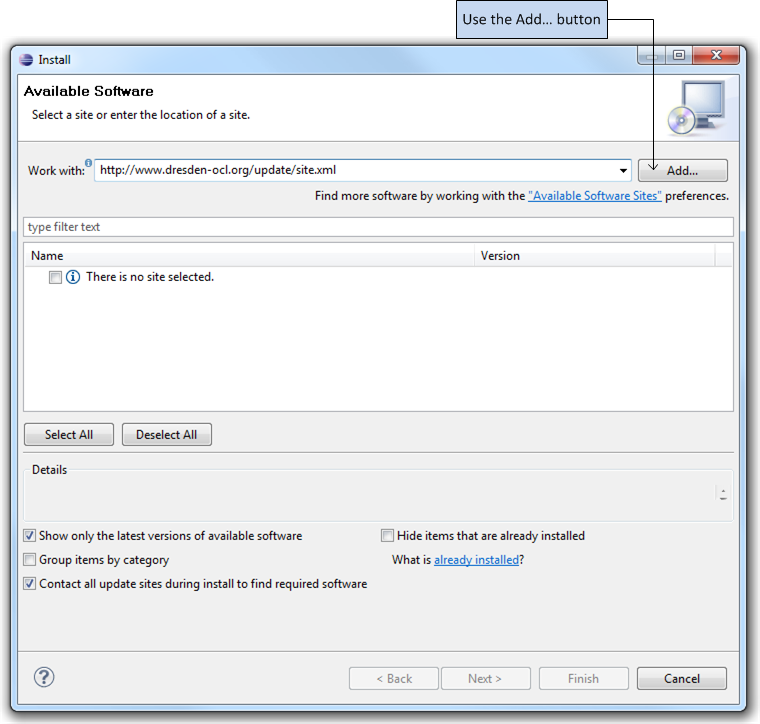
\includegraphics[width=0.8\linewidth]{figures/introduction/updateSite01}
	\caption{Adding an Eclipse Update Site (Step 1).}
	\label{pic:intro:updateSite01}

  \vspace{2.0em}
  
	\centering
	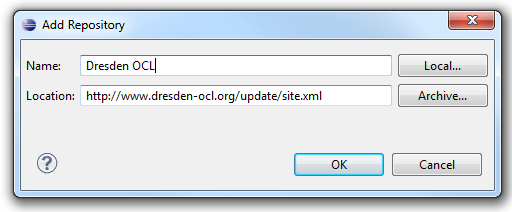
\includegraphics[width=0.6\linewidth]{figures/introduction/updateSite02}
	\caption{Adding an Eclipse Update Site (Step 2).}
	\label{pic:intro:updateSite02}
\end{figure}

Now you can select the features of \acl{DOT4Eclipse} which you want to install. 
Select them and click on the \eclipse{Next >} button (see 
Figure~\ref{pic:intro:updateSite03}). An overview about all features of 
\acl{DOT4Eclipse} can be found in Table~\ref{tab:plugins} in the appendix of 
this manual. Follow the wizard and agree with the user license. Then DresdenOCL
will be installed. Afterwards, you should restart your Eclipse application to 
finish the installation.

\begin{figure}[t]
	\centering
	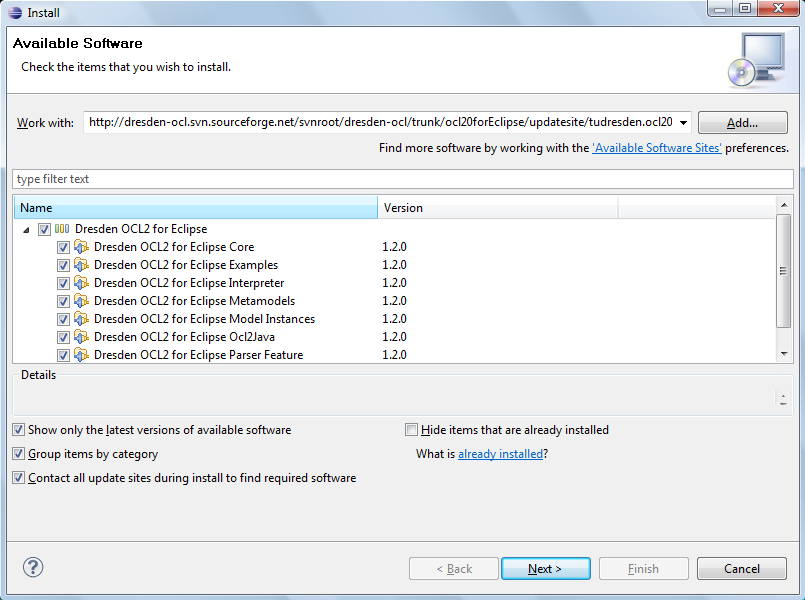
\includegraphics[width=1.0\linewidth]{figures/introduction/updateSite03}
	\caption{Selecting features of Dresden OCL2 for Eclipse.}
	\label{pic:intro:updateSite03}
\end{figure}
	
	
	
\subsection{Importing Dresden OCL2 for Eclipse from the SVN}

To use \acl{DOT4Eclipse} by checking out the source code from the \acs{SVN} you
need to install an \acs{SVN} client. In the following we use the 
\keyword{Eclipse Subversive} plug-in and at least one of the \keyword{\acs{SVN}
Connectors} available at~\cite{WWW:eclipseSubversive}.

After installing Eclipse Subversive, a new \keyword{Eclispe Perspective} 
providing access to \acs{SVN} should exist. The perspective can be opened via 
the menu \eclipse{Window > Open Perpective > Other... > SVN Repository
Exploring}. In the view \eclipse{\acs{SVN} Repositories} you can add a new 
repository using the \acs{URL} 
\url{https://dresden-ocl.svn.sourceforge.net/svnroot/dresden-ocl/} (see 
Figure~\ref{pic:intro:svn01}).

\begin{figure}[!b]
	\centering
	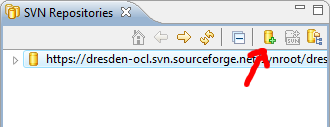
\includegraphics[width=0.5\linewidth]{figures/introduction/svn01}
	\caption{Adding an SVN repository.}
	\label{pic:intro:svn01}
\end{figure}

After pushing the \eclipse{Finish} button, the \acs{SVN} repository root should 
be visible in the \eclipse{\acs{SVN} Repositories} view. To checkout the
plug-ins, you have to select them in the repository directory 
\reference{trunk/ocl20\-for\-Eclipse/eclipse} and use the \eclipse{Checkout...} 
function in the context menu (see Figure \ref{pic:intro:svn02}).
	
\begin{figure}[!t]
	\centering
	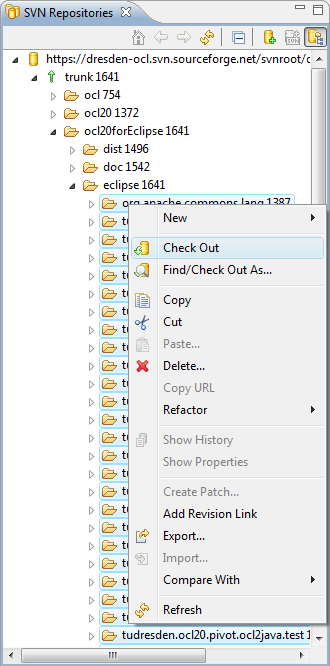
\includegraphics[width=0.5\linewidth]{figures/introduction/svn02}
	\caption{Checkout of the Dresden OCL2 Toolkit plug-in projects.}
	\label{pic:intro:svn02}
\end{figure}


\subsection{Which Plug-ins do You need at least?}

Often people wonder which plug-ins of \acl{DOT4Eclipse} they require for a
minimum installation. The answer to this question depends on the things you 
plan to do with \acl{DOT4Eclipse}. Table~\ref{tab:plugins} in the appendix of 
this manual shows a list of the currently existing plug-ins of
\acl{DOT4Eclipse}, that are related to different features. You should install 
at least the \keyword{Core} feature, at least one meta-model of the 
\keyword{Meta-Models} feature, and the complete \keyword{Parser} feature. The 
\keyword{Interpreter} and \keyword{OCL22Java} features are only required if you 
want to interpret constraints or to generate code from constraints,
respectively. If you import or interpret model instances, you need to install 
the \keyword{Model Instances} feature as well. The examples of the 
\keyword{Example} feature are only required to run the examples provided in 
this manual. We recommend to install all provided features.
		


\subsection{Building the OCL2 Parser}
\todomt{Revise this section and adapt it to the new OCL Editor/Parser.}	
If you decided to run \acl{DOT4Eclipse} as source code plug-ins from an Eclipse work\-space, you need to build the \keyword{OCL2 Parser} via an \keyword{Ant} build script. If you installed the Toolkit using the update site, you can skip this section.
  
To build the \acs{OCL} Parser select the file \reference{build.xml} in the project \reference{tudresden.\linebreak[0]ocl20.pivot.ocl2\-par\-ser} and open the context menu. Select the function \eclipse{Run As ... > Ant Build ...} (see Figure~\ref{pic:intro:parserbuild01}).

\begin{figure}[p]
	\centering
	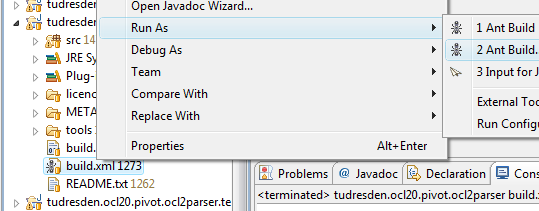
\includegraphics[width=0.8\linewidth]{figures/introduction/parserbuild01}
	\caption{Executing the OCL2 Parser build script.}
	\label{pic:intro:parserbuild01}

  \vspace{4.0em}

	\centering
	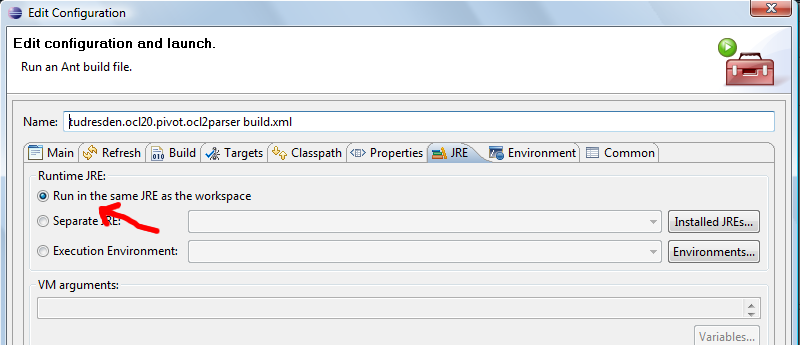
\includegraphics[width=0.8\linewidth]{figures/introduction/parserbuild02}
	\caption{Settings of the JRE for the Ant build script.}
	\label{pic:intro:parserbuild02}

  \vspace{4.0em}

	\centering
	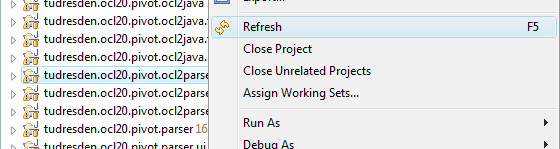
\includegraphics[width=0.8\linewidth]{figures/introduction/parserbuild03}
	\caption{Refreshing the project ``tudresden.ocl20.pivot.oclparser''.}
	\label{pic:intro:parserbuild03}
\end{figure}
	
A new window should open. Switch to the tab \keyword{\acs{JRE}}, select the check box \keyword{Run in the same \acs{JRE} as the workspace} and push the \keyword{OK} button (see Figure~\ref{pic:intro:parserbuild02}). Afterwards, the \acs{OCL}2 Parser should be generated without errors. If an error like ``Unable to find javac compiler.'' occurs, you might be trying to run the \keyword{Ant} script with a \keyword{\acl{JRE}} instead of a \keyword{\acs{JDK}} (For errors like this one) use the \eclipse{Installed JREs...} button in the same window to select a \acs{JDK} instead.
	
After executing the build script successfully you need to update the projects in your workspace. Update the project \reference{tudresden.ocl20.pivot.oclparser} via context menu (\eclipse{Refresh}, see Figure~\ref{pic:intro:parserbuild03}).
	
Additionally, you need to recompile all depending projects. Select the function \eclipse{Project > Clean...~> Clean all projects} in the Eclipse menu to clean all projects. Now all the projects should not contain any errors any more and should be executable.



\section{Loading Models, Model Instances and Constraints}

If you installed the \acl{DOT4Eclipse} using the update site, you can execute
the toolkit by re-starting your Eclipse distribution. If you imported the
Toolkit as source code plug-ins into an Eclipse workspace, you have to start a 
new Eclipse instance. You can start a new instance via the menu \eclipse{Run >
Run As > Eclipse Application}. If the menu \eclipse{Eclipse Application} is not 
available or disabled you need to select one of the plug-ins of the toolkit in
the \eclipse{Package Explorer} first.


\subsection{The Simple Example}
\label{intro:simpleExample}

The use of \acl{DOT4Eclipse} is explained using the \keyword{Simple Example} 
which is located in the plug-in 
\reference{tudresden.ocl20.pivot.examples.\linebreak[0]simple}. 
Figure~\ref{pic:examples:simple01} shows a class diagram of the Simple Example.

\begin{figure}[!htbp]
	\centering
	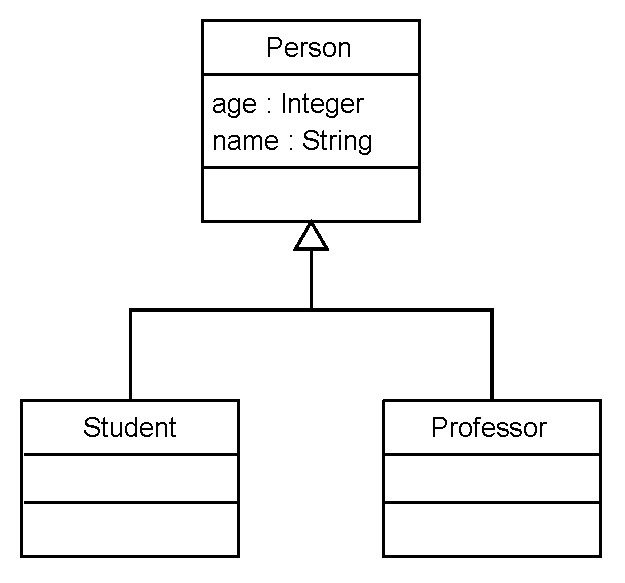
\includegraphics[width=0.5\linewidth]{figures/examples/simple01}
	\caption{A class diagram describing the Simple Example model.}
	\label{pic:examples:simple01}
\end{figure}

\acl{DOT4Eclipse} provides more examples than the Simple Example. The different 
examples use different meta-models which is possible with the \textit{Pivot
Model} architecture of the Toolkit. An overview about all examples provided 
with \acl{DOT4Eclipse} is listed in Table~\ref{tab:examples} in the appendix of
this manual. The Simple Example can be used with two different meta-models. 
These are \keyword{\acs{UML} 2.0} (based on \keyword{\acs{Eclipse MDT} 
\acs{UML}}) and \keyword{Java}.
	

\subsection{Loading a Model}
	
After starting Eclipse you have to load a model into DresdenOCL. If the 
plug-ins of \acl{DOT4Eclipse} have been installed using the update site, the 
Simple Example plug-in has to be imported into the \keyword{Workspace} first. 
Create a new Java project into your workspace and select the \keyword{Import
Wizard} \eclipse{General > Archive File}. In the following window select the 
\eclipse{plugins} directory in your Eclipse root folder, select the archive 
\reference{tudresden.ocl20.pivot.examples.\linebreak[0]simple\_<version\_nr>.jar}
and push the \eclipse{Finish} button.

Now you can load a model. Select the menu option \eclipse{Dresden OCL2 > Load 
Model}. In the opened wizard you have to select a model file and a meta-model 
for the model\footnote{Section~\ref{sect:info:models} gives an overview over 
the different meta-models supported by DresdenOCL.} (see 
Figure~\ref{pic:intro:loadmodel01}). Push the button \eclipse{Browse 
Workspace...} and select the file \reference{model/simple.uml} inside the 
Simple Example Project. Then select the meta-model \acs{UML}2 and push the 
\eclipse{Finish} button.

Figure~\ref{pic:intro:loadmodel02} shows the loaded Simple Example model, which
uses \acs{UML}2 as its meta-model. Via the menu button of the \eclipse{Model 
Browser} (the little triangle in the right top corner) you can switch between 
different models loaded into \acl{DOT4Eclipse} (see 
Figure~\ref{pic:intro:loadmodel03}) With the two circled arrows icon you can
reload a model into DresdenOCL, with the red \emph{X} you can close the
currently selected model.
	
\begin{figure}[!htbp]
	\centering
	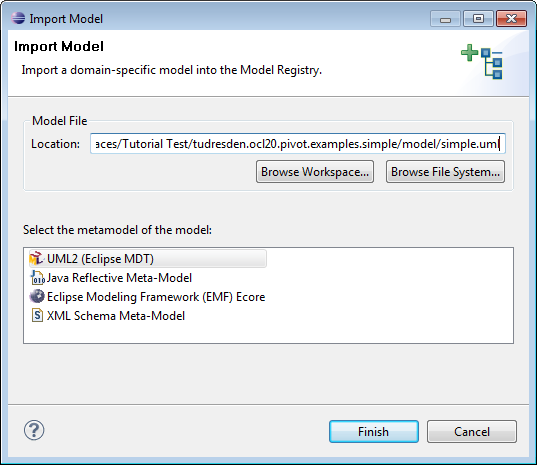
\includegraphics[width=0.7\linewidth]{figures/introduction/loadmodel01}
	\caption{Loading a Model.}
	\label{pic:intro:loadmodel01}
	
  \vspace{6.0em}

	\centering
	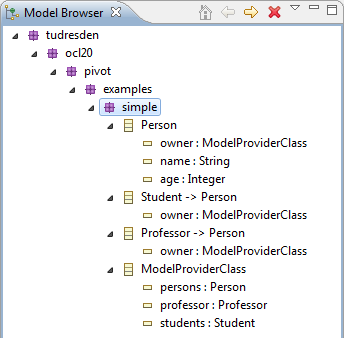
\includegraphics[width=0.4\linewidth]{figures/introduction/loadmodel02}
	\caption{The Simple Example Model in the Model Browser.}
	\label{pic:intro:loadmodel02}
\end{figure}

	
\subsection{Loading a Model Instance}
\label{intro:loadModel}
	
After loading a model, you can load a an instance of this model using another 
wizard. The model instance is required to interpret OCL constraints on
elements instantiating the classes described in the opened model. Which kinds
of model instances are supported in DresdenOCL is documented in
Section~\ref{sect:info:modelinstances}. Use the menu option \eclipse{Dresden 
OCL2 > Load Model Instance}. In the opened wizard you have to select a model 
instance (in this tutorial we used the file 
\reference{bin/tudresden/ocl20/\linebreak[0]pivot/examples/\linebreak[0]sim\-ple/\linebreak[0]in\-stance/\linebreak[0]Mo\-del\-InstanceProviderClass\linebreak[0].class}
of the Simple Example (see Figure~\ref{pic:intro:loadInstance01}). Besides the
model instance resource you have to select a model for which the model instance 
shall be loaded and the type of model instance you want to load (we want to 
load a \keyword{Java Instance}).

\begin{figure}[!p]
	\centering
	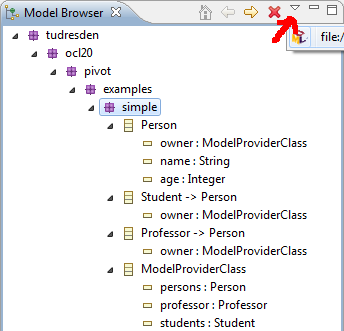
\includegraphics[width=0.4\linewidth]{figures/introduction/loadmodel03}
	\caption{You can switch between different Models using the little Triangle.}
	\label{pic:intro:loadmodel03}

  \vspace{6.0em}
  
	\centering
	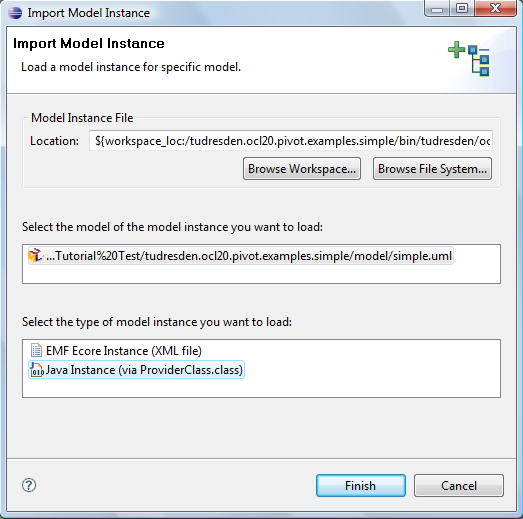
\includegraphics[width=0.7\linewidth]{figures/introduction/loadinstance01}
	\caption{Loading a Simple Model Instance.}
	\label{pic:intro:loadInstance01}
\end{figure}

Figure~\ref{pic:intro:loadInstance02} shows the imported model instance. Like
in the model browser you can switch between different model instances and you 
can close selected instances. Note that the \eclipse{Model Instance Browser} 
only shows the model instances of the model actually selected in the model 
browser. By switching the model in the model browser, you also switch the pool 
of model instances available in the model instance browser.

\begin{figure}[!t]
	\centering
	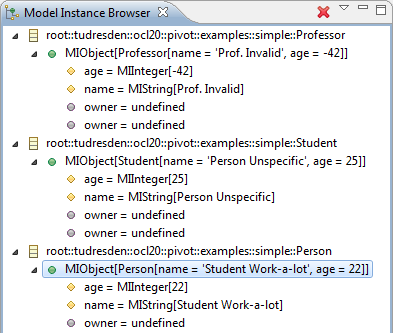
\includegraphics[width=0.6\linewidth]{figures/introduction/loadinstance02}
	\caption{A simple model instance in the Model Instance Browser.}
	\label{pic:intro:loadInstance02}
\end{figure}
	
	
\subsection{Parsing OCL Expressions}
\label{intro:oclEditor}
\todomt{Revise this Section and adapt it to the new OCL Editor.}	
Before you can work with \acs{OCL} constraints, you have to load them like the model and the model instance into DresdenOCL. Use the menu option \eclipse{Dresden OCL2 > Parse OCL Constraints} and select an \acs{OCL} file. In this tutorial we use the \acs{OCL} file \reference{constraints/invariants.ocl} of the Simple Example. (see Figure \ref{pic:intro:loadconstraints01}). The constraints of the file \reference{constraints/invariants.ocl} are shown in Listing \ref{list:intro:constraints01}.

The expressions of the selected \acs{OCL} file are parsed and added to the actually selected model. Figure~\ref{pic:intro:loadconstraints02} shows the \eclipse{Model Browser} containing the model and the parsed expressions. Using the icons depicted in Figure~\ref{pic:intro:loadconstraints03}, you can remove selected or all parsed OCL constraints from the model again.

\begin{figure}[b]	
\lstset{
  language=OCL
}
\begin{lstlisting}[caption={The invariants of the simple examples.}, captionpos=b, label=list:intro:constraints01]
package tudresden::ocl20::pivot::examples::simple

-- The age of Person can't be negative.
context Person
inv: age >= 0

-- Students should be 16 or older.
context Student
inv: age > 16

-- Proffesors should be at least 30.
context Professor
inv: not (age < 30)

endpackage
\end{lstlisting}
\end{figure}

\begin{figure}[p]
	\centering
	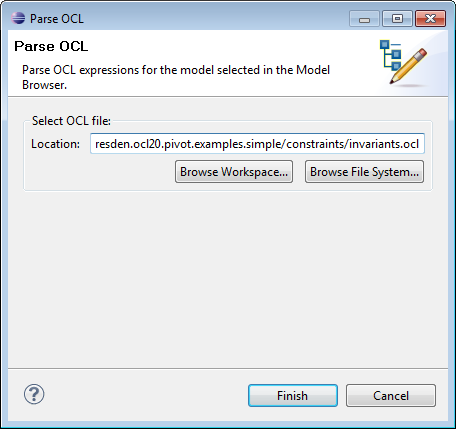
\includegraphics[width=0.6\linewidth]{figures/introduction/loadconstraints01}
	\caption{The import of OCL expressions.}
	\label{pic:intro:loadconstraints01}
	
	\vspace{3.0em}
	
	\centering
	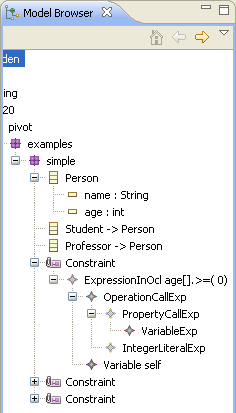
\includegraphics[width=0.5\linewidth]{figures/introduction/loadconstraints02}
	\caption{Parsed expressions and the model in the Model Browser.}
	\label{pic:intro:loadconstraints02}
\end{figure}
	
\begin{figure}[t]
	\centering
	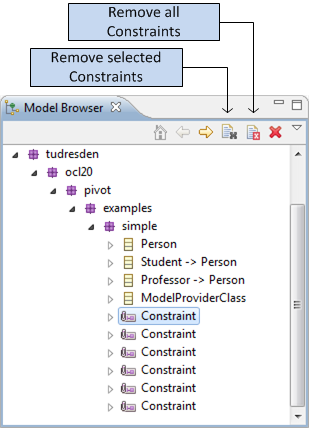
\includegraphics[width=0.4\linewidth]{figures/introduction/loadconstraints03}
	\caption{How to remove Constraints from a Model again.}
	\label{pic:intro:loadconstraints03}
\end{figure}
	
	

\section{Summary}
  
This chapter described how to use \acl{DOT4Eclipse}. It explained how to 
install the plug-ins of \acl{DOT4Eclipse}. Afterwards, the import of models,
model instances and \acs{OCL} constraints into DresdenOCL was explained.

Now, the imported models can be used with the tools provided by DresdenOCL. For
example you can use the \keyword{OCL Interpreter} to interpret \acs{OCL} 
constraints for a given model and model instance (as explained in 
Chapter~\ref{chapter:interpretation}) or you can use the \keyword{OCL22Java
Code Generator} to generate \keyword{AspectJ} code for a loaded model and 
\acs{OCL} constraints (as explained in Chapter~\ref{chapter:codeGeneration}).
\todocw{Mention OCL22SQL here when available.}

If you do not want to use Eclipse, but still want to interpret OCL constraints 
or generate AspectJ code, you can use DresdenOCL as a stand-alone library
outside of Eclipse. A detailed description on how to do this is given in 
Chapter~\ref{chapter:standalone}.
